\chapter{System Concept}\label{chap:concept}
This chapter will cover the system concept, functionality that it offers and general functional system description. It should clarify how the SmartNotes can be used, illustrate their design using the UML diagrams and prepare the reader for more detailed system description included in the chapter~\ref{chap:sys_description}.

The idea of SmartNotes came by inspiration of Google Notebook application which was actively developed until January 2009 where the Google announced that further development work on this project is stopped. It has a great interface and nice features were some of them were motioned in section~\ref{subsec:google_notebook} what still was missing was comfortable notes usage without the network connectivity. The aim was to use the idea of making a truly scalable notes taking application that would be even more flexible.

\section{Functionality description}\label{sec:functionality_descr} 
Description of how the the system can be used should by highly important both to the developer and to the end user. It helps to get a general perspevive called 10,000-foot view\cite[page 49]{uml_use_case} of the system which and make useful observations. The implementation, conceptual and system design decisions are on the third plane what counts is what final functionality will it offer. For that reason use case scenarios and flow charts will be very helpful in describing the efficient way of using the SmartNotes application.

Users willing to work on their notes disregarding the network connectivity will need to install iSmartNotes which is a graphical interface to the SmartNotes. That means that the SmartNotes application is divided into the web based system and the graphical the desktop interface. With that separation some UI experiments can be done and the user does not to have the web browser opened to work on the notes. The web based part of SmartNotes makes the synchronization feature possible. It also allows to monitor the entire system of SmartNotes. However to use the synchronization feature the iSmartNotes needs to get activated by the user. Because users of SmartNotes are expected to have a Google account\footnote{Creating a Google account by visiting \url{https://www.google.com/accounts/} gives a access to various services offered by Google company where Gmail, Google News or Google Finance ore one of the most popular.This is a secure and solid service that users can relay on.} the activation code will be available after login to SmartNotes system with that account. This process is illustrated on the the figure~\ref{fig:ismartnotes_activation}. The idea behind it is to make the use of the popular Google Account and not multiply the accounts to services that the user has to know the login and password. Basing on the activation key the user get access to his personalized SmartNotes account and to synchronization feature. Without activation iSmartNotes can be used as a regular notes editor.  
\begin{figure}[ht]
\begin{center}
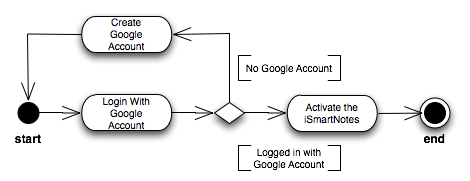
\includegraphics[scale=0.6]{charts/activate_iSmartNotes.png}
\caption{The iSmartNotes application activation with the Google Account.}
\label{fig:ismartnotes_activation}
\end{center}
\end{figure}
The skim of functionality offered by iSmartNotes is demonstrated on figure~\ref{fig:workon_ismartnotes}.
\begin{figure}[ht]
\begin{center}
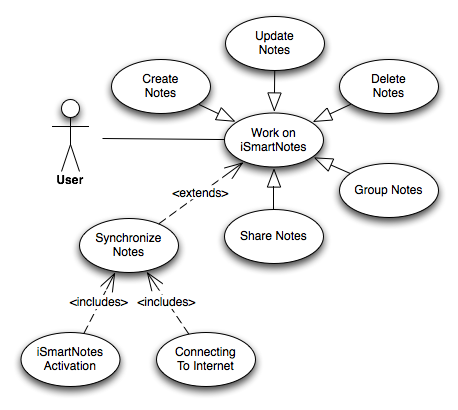
\includegraphics[scale=0.5]{charts/work_on_iSmartNotes.png}
\caption{The iSmartNotes application use cases.}
\label{fig:workon_ismartnotes}
\end{center}
\end{figure}
This includes the CRUD operations and three extra features. The notes can be easily grouped together in named tabs. This should make organizing and finding notes much easier. Secondly it should be possible to publish the notes marked as shared. Finally the synchronization feature that requires iSmartNotes activation and network connection to contact with the web based part of SmartNotes. What needs to be discussed is the cooperation between those two parts iSmartNotes and web based part of SmartNotes. The relation between them and the functionality offered to the user and administrator are shown on figure~\ref{fig:ismartnotes_smartnotes}. 
\begin{figure}[ht]
\begin{center}
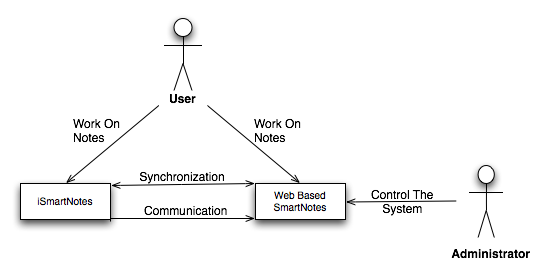
\includegraphics[scale=0.5]{charts/iSmartNotes_SmartNotes.png}
\caption{The cooperation of iSmartNotes and web based SmartNotes.}
\label{fig:ismartnotes_smartnotes}
\end{center}
\end{figure}

It is interesting concept to allow the user work on iSmartNotes and on the Web based part of SmartNotes exchangeably  and letting the SmartNotes application care for work synchronization. This was also marked on the discussed picture. However that is a remark of what could be done to make the application more functional and elastic but the user functionality of the web interface of realized project will be mineralized. On the Other hand administrator will get the access to such a tools like datastore data browser, system status or application dashboard described in section~\ref{sec:gae_general}. This can help to fast diagnose that something is going not right with the application and rollback it to the latest stable version. Moreover  it can indicate that the rescuers are not sufficient to serve the traffic and eventually extend them. Those tools work great with cooperation with Google Webmaster Tools and the Google Analytics as they can provide more information concerning the web page and its visitors.

Some additional explanations requires the synchronization feature. It will be realized by the version control system which were introduced in section~\ref{sec:popular_vcs}. No matter if the user works online or not he will have the full access to his notes and when he can use Internet notes can become synchronized. As marked on the graph from figure~\ref{fig:ismartnotes_smartnotes} the synchronization process is bidirectional from the web based part of SmartNotes which plays a role of main server and the iSmartNotes playnig the role of clients and reverse. That should allow to update the notes which could be for example edited just before leaving the office or push the just added list of things to do after coming from vacation. Next thing marked on the graph from figure~\ref{fig:ismartnotes_smartnotes} is the one directional communication between iSmartNotes and SmartNotes which should be understand as a additional logic allowing the to perform some operations on the user side by the help of iSmartNotes. That should include displaying the user information's about some important events like availability of new feature or information about availability of newer version.  Its one directional as it will be iSmartNotes application which will be in order to get this informations from the SmartNotes server and display it to the user. The presented functionality definitely does not fully exploit the possible feature list but as mentioned in section~\ref{subsec:vcs_comparison} it is a good practice to keep the application as simple as possible and focus on a set of clearly defined key features.
\section{Functional description}\label{sec:functional_descr}
The SmartNotes application should run on a infrastructure that can ensure high availability and be ready to handle high load. Assuring easy system maintenance and availability for future expanding wold be also strongly desirable features. It is not pointless to mention that all this features use resources what means that financial model is really on importance. That are is developer 10,000-foot view for the system requirements.
Users should get well informed about it, what it does and shout be able to easily start to use SmartNotes. For this reason the landing page should be informal with and support make it easy to get started. It would be best it it wold be international to reach greater group of users.

From the architectural point of view SmartNotes is though as a simple client-server application. The only one small difference is that the SmartNotes application uses DVCS which makes all the machines access same set of commands and make their hard disks hold the entire repository with it history. It may be confusing that it still remains a client-server architecture. In dead it is a little strange but just like centralized VCS don't know any other architecture than client-server the distributed version control use it as one of possible use cases. In that case one of the machines fulfills a role of reverential server to which all remaining machines direct its requests. It is a kind of public repository that holds most recent version.

